\documentclass[]{article}
\usepackage{lmodern}
\usepackage{amssymb,amsmath}
\usepackage{ifxetex,ifluatex}
\usepackage{fixltx2e} % provides \textsubscript
\ifnum 0\ifxetex 1\fi\ifluatex 1\fi=0 % if pdftex
  \usepackage[T1]{fontenc}
  \usepackage[utf8]{inputenc}
\else % if luatex or xelatex
  \ifxetex
    \usepackage{mathspec}
  \else
    \usepackage{fontspec}
  \fi
  \defaultfontfeatures{Ligatures=TeX,Scale=MatchLowercase}
\fi
% use upquote if available, for straight quotes in verbatim environments
\IfFileExists{upquote.sty}{\usepackage{upquote}}{}
% use microtype if available
\IfFileExists{microtype.sty}{%
\usepackage{microtype}
\UseMicrotypeSet[protrusion]{basicmath} % disable protrusion for tt fonts
}{}
\usepackage[margin=1in]{geometry}
\usepackage{hyperref}
\hypersetup{unicode=true,
            pdftitle={Chapter 7: Iterative Solvers},
            pdfborder={0 0 0},
            breaklinks=true}
\urlstyle{same}  % don't use monospace font for urls
\usepackage{graphicx,grffile}
\makeatletter
\def\maxwidth{\ifdim\Gin@nat@width>\linewidth\linewidth\else\Gin@nat@width\fi}
\def\maxheight{\ifdim\Gin@nat@height>\textheight\textheight\else\Gin@nat@height\fi}
\makeatother
% Scale images if necessary, so that they will not overflow the page
% margins by default, and it is still possible to overwrite the defaults
% using explicit options in \includegraphics[width, height, ...]{}
\setkeys{Gin}{width=\maxwidth,height=\maxheight,keepaspectratio}
\IfFileExists{parskip.sty}{%
\usepackage{parskip}
}{% else
\setlength{\parindent}{0pt}
\setlength{\parskip}{6pt plus 2pt minus 1pt}
}
\setlength{\emergencystretch}{3em}  % prevent overfull lines
\providecommand{\tightlist}{%
  \setlength{\itemsep}{0pt}\setlength{\parskip}{0pt}}
\setcounter{secnumdepth}{5}
% Redefines (sub)paragraphs to behave more like sections
\ifx\paragraph\undefined\else
\let\oldparagraph\paragraph
\renewcommand{\paragraph}[1]{\oldparagraph{#1}\mbox{}}
\fi
\ifx\subparagraph\undefined\else
\let\oldsubparagraph\subparagraph
\renewcommand{\subparagraph}[1]{\oldsubparagraph{#1}\mbox{}}
\fi

%%% Use protect on footnotes to avoid problems with footnotes in titles
\let\rmarkdownfootnote\footnote%
\def\footnote{\protect\rmarkdownfootnote}

%%% Change title format to be more compact
\usepackage{titling}

% Create subtitle command for use in maketitle
\providecommand{\subtitle}[1]{
  \posttitle{
    \begin{center}\large#1\end{center}
    }
}

\setlength{\droptitle}{-2em}

  \title{Chapter 7: Iterative Solvers}
    \pretitle{\vspace{\droptitle}\centering\huge}
  \posttitle{\par}
  \subtitle{Joseph Sepich}
  \author{}
    \preauthor{}\postauthor{}
    \date{}
    \predate{}\postdate{}
  

\begin{document}
\maketitle

{
\setcounter{tocdepth}{2}
\tableofcontents
}
\hypertarget{problem-1-comparing-various-methods}{%
\section{Problem 1 Comparing Various
Methods}\label{problem-1-comparing-various-methods}}

Solve the following system using the four methods. \[
\left(\begin{array}{ccc} 
4 & 3 & 0\\
3 & 4 & -1\\
0 & -1 & 4
\end{array}\right)
\left(\begin{array}{c} 
x_1 \\
x_2 \\
x_3
\end{array}\right) =
\left(\begin{array}{c}
24 \\
30 \\
-24
\end{array}\right)
\]

\hypertarget{a.-tridiagonal-gaussian-elimination}{%
\subsection{a. Tridiagonal Gaussian
elimination}\label{a.-tridiagonal-gaussian-elimination}}

Step 1: \(a_1 = a_1 / 4\) \[
\left(\begin{array}{ccc} 
1 & 0.75 & 0\\
3 & 4 & -1\\
0 & -1 & 4
\end{array}\right)
\left(\begin{array}{c} 
x_1 \\
x_2 \\
x_3
\end{array}\right) =
\left(\begin{array}{c}
6 \\
30 \\
-24
\end{array}\right)
\]

Step 2: \(a_2 = a_2 - 3a_1\)

\[
\left(\begin{array}{ccc} 
1 & 0.75 & 0\\
0 & 1.75 & -1\\
0 & -1 & 4
\end{array}\right)
\left(\begin{array}{c} 
x_1 \\
x_2 \\
x_3
\end{array}\right) =
\left(\begin{array}{c}
6 \\
12 \\
-24
\end{array}\right)
\]

Step 3: \(a_2 = a_2 / 1.75\) \[
\left(\begin{array}{ccc} 
1 & 0.75 & 0\\
0 & 1 & -1.75\\
0 & -1 & 4
\end{array}\right)
\left(\begin{array}{c} 
x_1 \\
x_2 \\
x_3
\end{array}\right) =
\left(\begin{array}{c}
6 \\
6.85714 \\
-24
\end{array}\right)
\]

Step 4: \(a_1 = a_1 - 0.75a_2\)

\[
\left(\begin{array}{ccc} 
1 & 0 & 0.42857\\
0 & 1 & -1.75\\
0 & -1 & 4
\end{array}\right)
\left(\begin{array}{c} 
x_1 \\
x_2 \\
x_3
\end{array}\right) =
\left(\begin{array}{c}
0.85714 \\
6.85714 \\
-24
\end{array}\right)
\]

Step 5: \(a_3 = a_3+a_2\)

\[
\left(\begin{array}{ccc} 
1 & 0 & 0.42857\\
0 & 1 & -1.75\\
0 & 0 & 3.4285714
\end{array}\right)
\left(\begin{array}{c} 
x_1 \\
x_2 \\
x_3
\end{array}\right) =
\left(\begin{array}{c}
0.85714 \\
6.85714 \\
-17.14285714
\end{array}\right)
\]

Step 6: \(a_3 = a_3 / 3.4285714\)

\[
\left(\begin{array}{ccc} 
1 & 0 & 0.42857\\
0 & 1 & -1.75\\
0 & 0 & 1
\end{array}\right)
\left(\begin{array}{c} 
x_1 \\
x_2 \\
x_3
\end{array}\right) =
\left(\begin{array}{c}
0.85714 \\
6.85714 \\
-5
\end{array}\right)
\]

Step 7: \(a_1= a_1-0.42857a_3\) \[
\left(\begin{array}{ccc} 
1 & 0 & 0\\
0 & 1 & -1.75\\
0 & 0 & 1
\end{array}\right)
\left(\begin{array}{c} 
x_1 \\
x_2 \\
x_3
\end{array}\right) =
\left(\begin{array}{c}
3 \\
6.85714 \\
-5
\end{array}\right)
\]

Step 8: \(a_2 = a_2 + a_3/1.75\)

\[
\left(\begin{array}{ccc} 
1 & 0 & 0\\
0 & 1 & 0\\
0 & 0 & 1
\end{array}\right)
\left(\begin{array}{c} 
x_1 \\
x_2 \\
x_3
\end{array}\right) =
\left(\begin{array}{c}
3 \\
4 \\
-5
\end{array}\right)
\]

\hypertarget{b.-jacobis-method}{%
\subsection{b. Jacobi's Method}\label{b.-jacobis-method}}

Here we iterate on the vector x, setting it equal each time to the
solution of our guess and it's equation. Our iteration scheme is:

\[x_1^{k+1} = \frac1{4}(24-3x_2^k)\]
\[x_2^{k+1}= \frac1{4}(30-3x_1^k+x_3^k)\]
\[x_3^{k+1}=\frac1{4}(-24+x_2^k)\]

Let's start with the vector \(x^0=[6, 7.5, -6]'\), which is the best
choice starting with a diagonally dominant matrix.

Iteration 1:

\[x^1=[0.375, 1.5, -4.125]\] \[x^2=[4.875, 6.1875, -5.625]\]

After 2 iterations we are not very accurate at all.

\hypertarget{c.-gauss-seidel-method}{%
\subsection{c. Gauss-Seidel Method}\label{c.-gauss-seidel-method}}

Here we iterate on the vector x, doing the same as Jacobi, but using our
new x values when we get them. Our iteration scheme is:

\[x_1^{k+1} = \frac1{4}(24-3x_2^k)\]
\[x_2^{k+1}= \frac1{4}(30-3x_1^{k+1}+x_3^k)\]
\[x_3^{k+1}=\frac1{4}(-24+x_2^{k+1})\]

Let's start with the vector \(x^0=[6, 7.5, -6]'\), which is the best
choice starting with a diagonally dominant matrix.

\[x^1=[0.375, 5.71875, -4.57031]\] \[x^2=[1.71094, 5.07422, -4.73145]\]

Here the x\textsubscript{3} value is already getting quite close to it's
actual value.

\hypertarget{d.-sor-method}{%
\subsection{d. SOR Method}\label{d.-sor-method}}

Here we iterate just like the previous Gauss-Seidel method, but give an
accelerant to the new value of x. Our iteration scheme is (using w =
1.25):

\[x_1^{k+1} =(1-w)x_1^k+ w\frac1{4}(24-3x_2^k) = (-0.25)x_1^k+ 1.25\frac1{4}(24-3x_2^k)\]
\[x_2^{k+1}= (1-w)x_2^k+ w\frac1{4}(30-3x_1^{k+1}+x_3^k)=(-0.25)x_2^k+ 1.25\frac1{4}(30-3x_1^{k+1}+x_3^k)\]
\[x_3^{k+1}=(1-w)x_3^k+ w\frac1{4}(-24+x_2^{k+1})=(-0.25)x_3^k+ 1.25\frac1{4}(-24+x_2^{k+1})\]

Let's start with the vector \(x^0=[6, 7.5, -6]'\), which is the best
choice starting with a diagonally dominant matrix.

\[x^1 = [-1.0313, 6.5918, -3.9401]\] \[x^2 = [1.578, 5.0164, -4.9474]\]

The value of x\textsubscript{3} is even closer than the previous two.
You can see such a noticable increase in the accuracy of the last
variable compared to the first two in this iteration and the
Gauss-Seidel over the Jacobi method, because the third variable is able
to use the new value obtained from the iteration already whereas
x\textsubscript{1} uses no new values and x\textsubscript{2} still uses
x\textsubscript{3}'s old value when you calculate them. You could also
clearly see the affect of having the over relaxtion technique.

\hypertarget{problem-2-sor-in-matlab}{%
\section{Problem 2 SOR in Matlab}\label{problem-2-sor-in-matlab}}

My Function:

\begin{verbatim}
function [x,nit]=sor(A,b,x0,w,d,tol,nmax)
% SOR : solve linear system with SOR iteration
% Usage: [x,nit]=sor(A,b,x0,omega,d,tol,nmax)
% Inputs:
%   A : an n x n matrix
%   b : the rhs vector, with length n
%   x0 : the start vector for the iteration% tol: error tolerance
%   w: relaxation parameter, (1 < w < 2),
%   d : band width of A.
% Outputs::
%   x : the solution vector
%   nit: number of iterations

D = diag(diag(A)); % first diag gets diag of A, second turns into diagonal matrix
L = tril(A)- D; % lower triangle, but remove the main diagonal
U = triu(A)- D; % upper triangle, but remove the main diagonal
 
% check for convergence of system with matrix norm of M
M = inv(D + w*L) * ( (1-w)*D - w*U);
y = inv(D + w*L)*b;
e= max(eig(M)); % L2 norm
if abs(e) >= 1
    disp ('Cannot converge with given parameters')
end

% set initial guess
x = zeros(length(b),nmax);
x(:,1) = x0;

nit = 1;
err1= norm(x(:,1)-b); %set intial error ||xk - xk-1|| <= tol, Axk - b <= tol
err2= norm(A*x(:,1)-b);
while err1 > tol & err2 > tol & nit <= nmax% go until nmax, within error tol for residual or xDiff norm
    x( : ,nit + 1 ) = y + M*x(:,nit);
    err1 = norm(x(:,nit+1)-x(:,nit));
    err2 = norm(A*x(:,nit+1)-b);
    nit = nit + 1;
end
 
fprintf ('The final ans obtaibed after %d iterations is  \n', nit)
x = x(:,nit-1);
disp(x);

end
\end{verbatim}

My Script

\begin{verbatim}
omega = 1.0:0.0001:1.9;
numIterations = zeros(length(omega),1);


% given inputs
A = ...
  [-2.011 1 0 0 0 0 0 0 0;
   1 -2.012 1 0 0 0 0 0 0;
   0 1 -2.013 1 0 0 0 0 0;
   0 0 1 -2.014 1 0 0 0 0;
   0 0 0 1 -2.015 1 0 0 0;
   0 0 0 0 1 -2.016 1 0 0;
   0 0 0 0 0 1 -2.017 1 0;
   0 0 0 0 0 0 1 -2.018 1;
   0 0 0 0 0 0 0 1 -2.019];

x = [0.95; 0.9; 0.85; 0.8; 0.75; 0.7; 0.65; 0.6; 0.55];
xResult = zeros(length(x),length(omega));


b = [-0.994974; 0.0015740700000000001; -0.00089667700000000013; -0.0027113700000000003; ...
     -0.00407407; -0.00511719; -0.00592917; -0.00657065; -0.507084];


for i = 1:length(omega)
    [xResult(:,i), numIterations(i)] = sor(A,b,x,omega(i),3,10^-4,100);
end

disp(numIterations)

figure
plot(omega, numIterations)
xlabel("Omega value of SOR")
ylabel("Iterations until convergence")
title("Omega value impact on convergence in SOR")

% After reviewing the plot 1.52 looks to be about the fastest value

sor(A,b,x,1.52,3,10^-4,100);
\end{verbatim}

My Figure

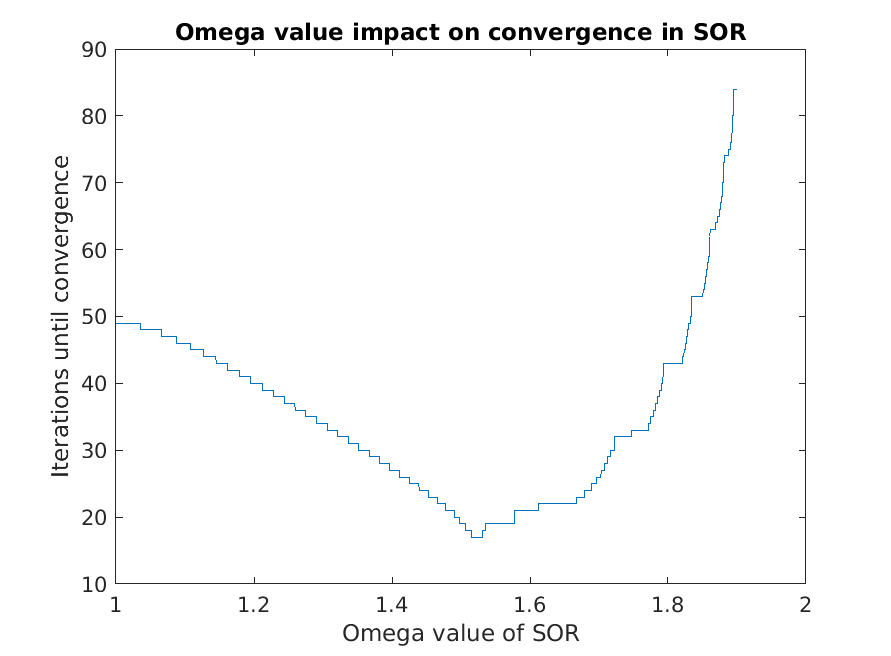
\includegraphics{./Problem2Fig.png}

My output from fastest convergence:

sor(A,b,x,1.52,3,10\^{}-4,100);

The final ans obtaibed after 17 iterations is

\begin{itemize}
\tightlist
\item
  0.598282174892330
\item
  0.548504459835072
\item
  0.506345876671595
\item
  0.470228835561903
\item
  0.438847388887656
\item
  0.411390422599940
\item
  0.387154972681848
\item
  0.365605562729382
\item
  0.346316779821866
\end{itemize}

It appears that having a value close to 1.5 is optimal, but it quickly
get's harder/less quick to converge after 1.5, versus a much less steep
slope in the decrease before the steep increase that we see.

\hypertarget{problem-3-jacobi-iterations-in-matlab}{%
\section{Problem 3 Jacobi Iterations in
Matlab}\label{problem-3-jacobi-iterations-in-matlab}}

My Function

\begin{verbatim}
function [x,nit] = jacobi(A,b,x0,tol,nmax)
%JACOBI Summary of this function goes here
%   Detailed explanation goes here
D = diag(diag(A)); % first diag gets diag of A, second turns into diagonal matrix
L = tril(A)- D; % lower triangle, but remove the main diagonal
U = triu(A)- D; % upper triangle, but remove the main diagonal
 
% check for convergence of system with matrix norm of M
M = -1 * inv(D)*(L + U);
y = inv(D)*b;
e= max(abs(eig(M))); % L2 norm
if abs(e) >= 1
    disp ('Cannot converge with given parameters')
end

% set initial guess
x = zeros(length(b),nmax);
x(:,1) = x0;

nit = 1;
err1= norm(x(:,1)-b); %set intial error ||xk - xk-1|| <= tol, Axk - b <= tol
err2= norm(A*x(:,1)-b);
while err1 > tol & err2 > tol & nit <= nmax% go until nmax, within error tol for residual or xDiff norm
    x( : ,nit + 1 ) = y + M*x(:,nit);
    err1 = norm(x(:,nit+1)-x(:,nit));
    err2 = norm(A*x(:,nit+1)-b);
    nit = nit + 1;
end
 
fprintf ('The final ans obtaibed after %d iterations is  \n', nit)
x = x(:,nit-1);
disp(x);
end
\end{verbatim}

My Script

\begin{verbatim}
% Set parameters
omega = 1.0:0.0001:1.9;
numIterations = zeros(length(omega),1);
tol = 10^-4;
nmax = 100;


% given inputs
A = ...
  [-2.011 1 0 0 0 0 0 0 0;
   1 -2.012 1 0 0 0 0 0 0;
   0 1 -2.013 1 0 0 0 0 0;
   0 0 1 -2.014 1 0 0 0 0;
   0 0 0 1 -2.015 1 0 0 0;
   0 0 0 0 1 -2.016 1 0 0;
   0 0 0 0 0 1 -2.017 1 0;
   0 0 0 0 0 0 1 -2.018 1;
   0 0 0 0 0 0 0 1 -2.019];

x = [0.95; 0.9; 0.85; 0.8; 0.75; 0.7; 0.65; 0.6; 0.55];
xResult = zeros(length(x),length(omega));


b = [-0.994974; 0.0015740700000000001; -0.00089667700000000013; -0.0027113700000000003; ...
     -0.00407407; -0.00511719; -0.00592917; -0.00657065; -0.507084];

jacobi(A,b,x,tol,nmax);
\end{verbatim}

Output

The final ans obtaibed after 84 iterations is

\begin{itemize}
\tightlist
\item
  0.909577773388009
\item
  0.834158809943258
\item
  0.770274149932905
\item
  0.715433109122108
\item
  0.667816804205437
\item
  0.626053655120232
\item
  0.589110712523574
\item
  0.556181082386154
\item
  0.526643205159853
\end{itemize}

This method took about as long as the longest convergence of the SOR
method. This method is definitely slower than SOR and I cannot see
anyway that Jacobi would be better, since SOR builds off of it.

\hypertarget{problem-4}{%
\section{Problem 4}\label{problem-4}}

Consider the following system.

\[
\left(\begin{array}{ccc} 
5 & 4 & -2\\
-2 & 8 & -3\\
1 & 1 & -7
\end{array}\right)
\left(\begin{array}{c} 
x \\
y \\
z
\end{array}\right) =
\left(\begin{array}{c}
2 \\
6 \\
5
\end{array}\right)
\]

\hypertarget{a.-perform-one-step-of-jacobi-iteration-with-starting-vector-111.}{%
\subsection{a. Perform one step of Jacobi iteration with starting vector
=
{[}1,1,1{]}.}\label{a.-perform-one-step-of-jacobi-iteration-with-starting-vector-111.}}

\[x^{k+1} = \frac15(2 - 4y^k + 2z^k)\]
\[y^{k+1} = \frac{1}8(6 + 2x^k + 3z)\]
\[z^{k+1} = -\frac17(5 - x^k - y^k)\]

Performing one step:

\[vector = [0, 0.875, -0.42857]\]

\hypertarget{b.-perform-one-step-of-gauss-seidel-iteration-with-startin-vector-111.}{%
\subsection{b. Perform one step of Gauss-Seidel iteration with startin
vector =
{[}1,1,1{]}.}\label{b.-perform-one-step-of-gauss-seidel-iteration-with-startin-vector-111.}}

\[x^{k+1} = \frac15(2 - 4y^k + 2z^k)\]
\[y^{k+1} = \frac{1}8(6 + 2x^{k+1} + 3z)\]
\[z^{k+1} = -\frac17(5 - x^{k+1} - y^{k+1})\]

Performing one step:

\[vector = [0, 1.125, -0.55357]\]

\hypertarget{c.-do-either-method-converge-on-this-system-why}{%
\subsection{c. Do either method converge on this system?
Why?}\label{c.-do-either-method-converge-on-this-system-why}}

Well we can take a look at both the actual evaluation of the sytem and
the norm of M in the matrix vector form. If we plug the equation into a
calculator we can find the actual value with Gaussian elimination to be
{[}0.186969, 0.569405, -0.606232{]}. You would expect the Gauss-Seidel
first iteration to be a better guess than the first Jacobi iteration,
but it is further off, so let's look at the value of the matrix norms.

Jacobi we have \(M = -D^{-1}(L+U)\) and G-S we have \(-(D + L)^{-1}U\).
Using a calculator we can see these norms are 0.50411 for the Jacobi
method and 0.20701 for the Gauss-Seidel method. That means that both
methods must converge.


\end{document}
